\documentclass[stu,12pt,floatsintext]{apa7}

%\usepackage[american]{babel}

\usepackage{csquotes} % One of the things you learn about LaTeX is at some level, it's like magic. The references weren't printing as they should without this line, and the guy who wrote the package included it, so here it is. Because LaTeX reasons.
\usepackage[T1]{fontenc} 
\usepackage{mathptmx} % This is the Times New Roman font, which was the norm back in my day. If you'd like to use a different font, the options are laid out here: https://www.overleaf.com/learn/latex/Font_typefaces
\usepackage[spanish,es-tabla]{babel}

\title{Clasificación de Microservicios para la persistencia y procesamiento de datos recolectados en tiempo real de sistemas embebidos del sector minero en el departamento de Boyacá}
\shorttitle{Clasificación de Microservicios para el sector minero}
\authorsnames{William Fernando Salamanca Barrera, Oscar Ricardo Guerrero Serna}

\authorsaffiliations{Universidad Pedagógica y Tecnológica de Colombia}
\course{Seminario de Trabajo de Grado 8108918} % LaTeX gets annoyed (i.e., throws a grumble-error) if this is blank, so I put something here. However, if your instructor will mark you off for this being on the title page, you can leave this entry blank (delete the PSY 4321, but leave the command), and just make peace with the error that will happen. It won't break the document.
\professor{PhD. Marco Javier Suarez Baron}  % Same situation as for the course info. Some instructors want this, some absolutely don't and will take off points. So do what you gotta.

\duedate{\today}

\abstract{Put your abstract here. In APA style, the abstract should be between 150 and 250 words depending on the journal.}
\begin{document}
	\maketitle
	\graphicspath{{./images/}}
	\renewcommand\contentsname{TABLA DE CONTENIDO}
	\tableofcontents
	
	\renewcommand\listfigurename{TABLA DE FIGURAS}
	\listoffigures
	\section{TEMA/TEMÁTICA}
	
	\begin{figure}[H]
		\centering
		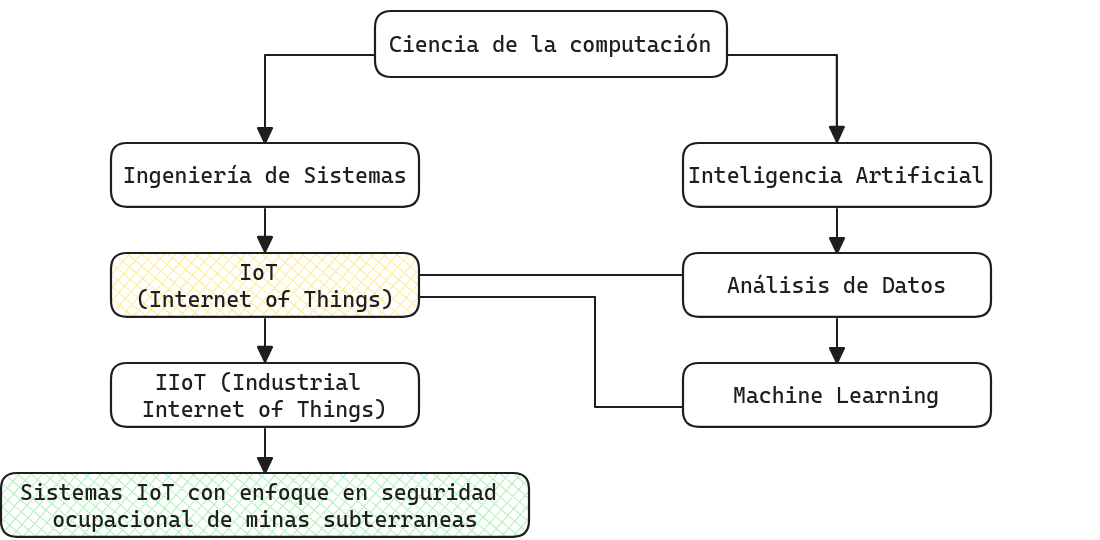
\includegraphics[scale=0.6]{mapa-conceptual}
		\captionsetup{justification=centering}
		\caption{Mapa conceptual del tema y la temática}
		\small
		Fuente: Autor
	\end{figure}
	\section{TITULO PROVISIONAL}
	Clasificación de Microservicios para un Sistema IoT de seguridad ocupacional en minas de la provincia de Sugamuxi del departamento de Boyacá.
	
	\section{PLANTEAMIENTO DEL PROBLEMA}
	\subsection{DESCRIPCIÓN DEL PROBLEMA}
	\subsubsection{Diagnostico}
	
	Se entienden a los sistemas IIoT (Industrial Internet of Things) como una aplicación de IoT (Internet of Things) en la industria. Concretamente en la industria minera durante los últimos años se ha presenciado una gran acogida de IoT en sus diferentes procesos de negocio. En lo que respecta a seguridad ocupacional, como preocupación primordial en la mayoría de las empresas,  los sensores IoT han sido cruciales para el monitoreo de condiciones ambientales. Sensores para la calidad del aire, la detección de gases nocivos para la salud así como para la detección de partículas de polvo producidos principalmente en el proceso de extracción de minerales, se encuentran entre las variables más comunes a monitorear por un sistema IoT con el fin de garantizar información en tiempo real que ayude a la toma de decisiones de prevención y gestión de emergencias\cite{reference-1}.
	
	Ante la problemática de recolección de datos provenientes de estos diferentes sensores, se identifica que sistemas como los SCADA (Supervisory Control and Data Acquisition)  que vienen siendo usados desde hace varios años, cubren la mayor parte de las necesidades que se presentan, pero surgen problemas asociados a esta alternativa, y es que los sistemas SCADA de tipo comercial tienen asociado un costo económico alto y problemas de compatibilidad.  Además, incluyendo los sistemas SCADA de uso libre, la arquitectura en la que se concibieron (cliente/servidor) no es la más optima para hacer frente a las demandas actuales de disponibilidad, fiabilidad, integridad, escalabilidad, rendimiento, seguridad, resiliencia, monitoreo y diagnostico.  Otro problema a resaltar es que estos sistemas operan a nivel de instalación, y el solo hecho de querer consumir los datos recogidos desde un cliente externo a la instalación, se presenta como un reto\cite{electronics8080822}. 
	 
	 Los diferentes sistemas que se encuentran implementados, la mayoría desde hace un par de décadas atrás, tienen una complejidad de integración inherente con los demás sistemas y sensores de la actualidad, esto debido al uso de stacks tecnológicos legacy y/o al uso de sensores específicos con un alto costo económico asociado a estos. Además de que son pocas las empresas que comparten datos respecto a cómo implementan su tecnología en el caso concreto de seguridad ocupacional\cite{iot1020029}.
	 
	 Adicionalmente son pocas las plataformas IoT que se encuentran en el mercado que cubren con las funcionalidades de analíticas de datos,  inteligencia artificial (AI) de propósito general o específicamente machine learning (ML), funcionalidades de visualización, interoperabilidad, captura de datos en tiempo real, gestión de dispositivos, que sean basados en la nube y que tengan una orientación a la industria minera. La mayoría de estas cubren parcialmente de forma satisfactoria algunas de estas funciones. Pero asociado a estas plataformas encontramos unas como ABB Ability que satisfacen muy bien todas las funcionalidades anteriormente mencionadas, con el inconveniente de que el adquirir este tipo de plataformas no es viable para medianas y pequeñas empresas de la provincia de Sugamuxi en el departamento de Boyacá debido a sus altos costos, y es que esas plataformas están concebidas para empresas mineras grandes \cite{iot-platforms}.

	\subsubsection{Pronostico}
	Ante la muy remota pero no nula probabilidad de optar por soluciones IoT costosas, las minas pueden empezar sufrir aumento en sus costos operativos, lo que trae una disminución de los margenes de ganancias, implicando reducción en la capacidad de re-inversión, afectando al crecimiento económico de la región con efectos como el aumento de la tasa de desempleo de los trabajadores involucrados directa e indirectamente en la cadena de producción. Además de presentarse una baja adopción en el uso de tecnología, lo cual también puede implicar que la empresa se quede resegada o hasta obsoleta frente a aquellas que si adoptan soluciones tecnológicas.
	
	Por otro lado, existe la posibilidad de que se opte por soluciones poco seguras y/o eficientes. Las cuales tienen asociadas una baja capacidad para escalar, poca seguridad y baja disponibilidad.
	
	Directamente puede que no opten por una, lo que afectaría directamente la toma de decisiones en cuestiones de seguridad para los trabajadores, junto con una  insuficiencia de recursos ante una muy probable baja eficiencia y productividad.
	\subsubsection{Control al pronostico}
	Ante esto se propone el diseño de un sistema IoT con un enfoque en seguridad ocupacional de minas en del departamento de Boyacá, asegurando principalmente un alto grado de cumplimiento en los siguientes atributos de calidad:
	
	\begin{itemize}
		\item Fiabilidad en la recolección de datos y emisión de alertas
		\item Disponibilidad 24/7
		\item Escabilidad principalmente asociada a la cantidad de datos que se recolectan por sistemas embebidos que amplíen los existentes.
		\item Mantenibilidad
		\item Seguridad principalmente en aspectos como la integridad, confidencialidad y disponibilidad de los datos.
		\item Rendimiento a nivel de recolección de datos, emisión de alertas
		\item Resiliencia 
		\item Monitoreo y diagnóstico
	\end{itemize}
	\subsection{FORMULACIÓN DEL PROBLEMA}
	\begin{itemize}
		   \item ¿Qué arquitecturas se encuentran consideradas en la industria minera para el desarrollo de sistemas IIoT?
		   \item ¿Cuáles son los estándares asociados a sistemas IoT en la industria minera?
			\item ¿En qué aspectos la arquitectura de microservicios se presenta como una mejor opción frente a las demás arquitecturas planteadas para este contexto?
	\end{itemize}
	
	\section{OBJETIVOS}
	\subsection{OBJETIVO GENERAL}
	¿Sistema a nivel de mina y nube?
	Diseñar un sistema IoT enfocado en la seguridad ocupacional para minas de la provincia de Sugamuxi del departamento de Boyacá.
	\subsection{OBJETIVOS ESPECÍFICOS}
	\begin{itemize}
		\item Analizar los diferentes modelos de transferencia de datos a nivel de capa de aplicación para sistemas embebidos.
		\item Identificar sensores y actuadores usados con enfoque de seguridad ocupacional en la industria minera.
		\item Determinar una clasificación de microservicios basada en las necesidades de seguridad ocupacional de minas en el departamento de Boyacá.
		\item Realizar pruebas de integración de los microservicios.
	\end{itemize}
	\section{JUSTIFICACIÓN}
		Por qué. De un conjunto de soluciones planteadas frente a una problemática, justificar, decir por qué se elige la solución n frente a las demás (ventajas, mejoras).
		
		En la industria minera encontramos los sistemas SCADA (Supervisory Control and Data Acquisition) con las características claves  de interfaz de usuario, pantallas gráficas, alarmas, tendencias, interfaces RTU (Unidades Terminales Remotas) y PLC (Controladores Lógicos Programables), escalabilidad, acceso a datos, bases de datos, redes, tolerancia a fallos y redundancia, procesamiento distribuido siguiendo la arquitectura cliente/servidor. Que aunque por muchos años ha servido en el proceso de recolección y procesamiento de datos a nivel general en la industria por varias décadas. Pero se presenta como una solución parcial dada su baja capacidad de interoperabilidad con otras partes interesadas como lo son otros sistemas, dispositivos, aplicativos usados por stakeholders \cite{SCADA_UMaT}.
		
		Para mitigar la carencia de sistemas legacy como el SCADA, muchas empresas en los últimos años han presentado al mercado soluciones basadas en IoT. Estas en su mayoría han probado ser opciones factibles debido a su implementación por parte de empresas mineras grandes. Pero estas diferentes soluciones convergen en pocos servicios por lo que se tienen soluciones diferentes que no están en la capacidad de cubrir con todas las necesidades requeridas, como el procesamiento de datos por parte de algoritmos de ML sin tener que sacrificar aspectos como el almacenamiento y el acceso a estos. Además de que, como estas soluciones son concebidas en el contexto de empresas mineras de países desarrollados, es poco viable que una mina en un país en vía de desarrollo puede llegar a costearla. También es importante mencionar que muchas de las solucione implementadas son software de propietario, que fueron desarrollados por la empresa para la empresa\cite{iot-platforms}.
		
		A partir de esto, se identifica que es necesario diseñar un sistema IoT con el enfoque de seguridad ocupacional, que cubras las necesidades especificas requeridas por el contexto de minas de la provincia de Sugamuxi en el departamento de Boyacá.
		
		Para qué. Para mejorar, adquirir...
		
		Se plantea por tanto una clasificación de microservicios que se ajuste a las necesidades del contexto, implementando un sistema IoT con tecnologias de código abierto para abaratar costos.
		
		Qué se busca. Validar, comprobar
		
		Por lo que se pretende validar que la solución planteada no sacrifica las caracteristicas planteadas en los sistemas anteriormente mencionados
		
		Cómo se busca. Explicación paso a paso (metodologia)
		Mediante la revisión de la literatura relacionada a diseño e implementación de sistemas IIoT en la industria minera, se pretende identificar caracteristicas que otorgan interoperabilidad entre sistemas a nivel de capa de aplicación. Luego de la identificación de sensores y actuadores implementados en minas subterráneas, se pretende plantear una clasificación de microservicios basado en estos y el contexto en el que se usan para finalmente integrarlo con un componente que permita la comunicación de estos.
		
		
		
	\section{DELIMITACIÓN Y ALCANCE}
	Detalle puntualmente en párrafos de mínimo 5 líneas cada una de las siguientes
	delimitaciones:
	- Por área geográfica:
	Según datos de la Agencia Nacional Minera, el departamento de Boyacá es el que encabeza las estadisticas de accidentalida de mortalidad en minas. Siendo casi que en su totalidad minas subterráneas dedicadas a la extracción de carbón
	- Por recursos:
	- Por tecnología
	
	Detalle puntualmente en párrafos de mínimo 5 líneas cada uno de los siguientes
	alcances de la investigación en lo relacionado a:
	- social,
	- humanístico,
	- educativo,
	- religioso,
	- cultural,
	- Tecnologica
	Hasta donde se llega en el proyecto
	
	\section{MARCO REFERENCIAL}
	\subsection{MARCO TEÓRICO}
	\subsection{MARCO CONCEPTUAL}
	Esta es una subsection de la Sección Uno\cite{mittelbach2004latex}
	\subsection{MARCO LEGAL}
	\subsection{MARCO HISTÓRICO}
	\subsection{MARCO METODOLÓGICO}
	
	\section{FUENTES DE INFORMACIÓN}
	
	\section{TIPO DE INVESTIGACIÓN}
	
	\section{CRONOGRAMA}
	
	\section{RECURSOS}
	\subsection{RECURSOS HUMANOS}
	\subsection{RECURSOS FÍSICOS}
	\subsection{RECURSOS TECNOLÓGICOS}
	
	\section{PRESUPUESTO}
	
	\section{BIBLIOGRAFÍA}
	\renewcommand\refname{Referencias}
	\bibliographystyle{apalike}
	\bibliography{./references.bib}
	
	

	
	
	\section{CONCLUSIONES}
	

\end{document}
